\chapter{Itération 1}

La méthodologie Scrum consiste à développer le produit incrémentalement, en
effet chaque itération résulte un prototype ayant des fonctionnalités du
produit demandé livrable. Le développement de ces fonctionnalités se fait
parallèlement puisque les membres de l'équipe avancent dans le même niveau
simultanément. Et ça nécessite de fixer un but commun de l'équipe et de faire
toutes les planifications nécessaires indispensables pour atteindre ce but.

\section{But de l'itération}

Dans le but de définir l'objectif et le périmètre fonctionnel de l'itération 1
et faire sa planification, tous les membres de l'équipe ont participé à une
réunion avec le Product Owner. Vue que l'équipe était encore débutante dans la
méthodologie Scrum et dans l'environnement de travail en équipe, un simple but
était tracé pour cette itération.

Le but de cette itération est de réaliser deux applications mobiles et web.
L'application mobile permet simplement de localiser instantanément
l'utilisateur et l'application web montre sa position géographique actuelle
continuellement sur une cartographie avec un marqueur. La
figure~\ref{fig:sprint1-prototype} représente un prototype du produit à
développer.

Pour éteindre ce but, une planification détaillée des tâches a était donnée
durant une réunion de trois heures de travail commun.

\begin{figure}[H]
    \centering
    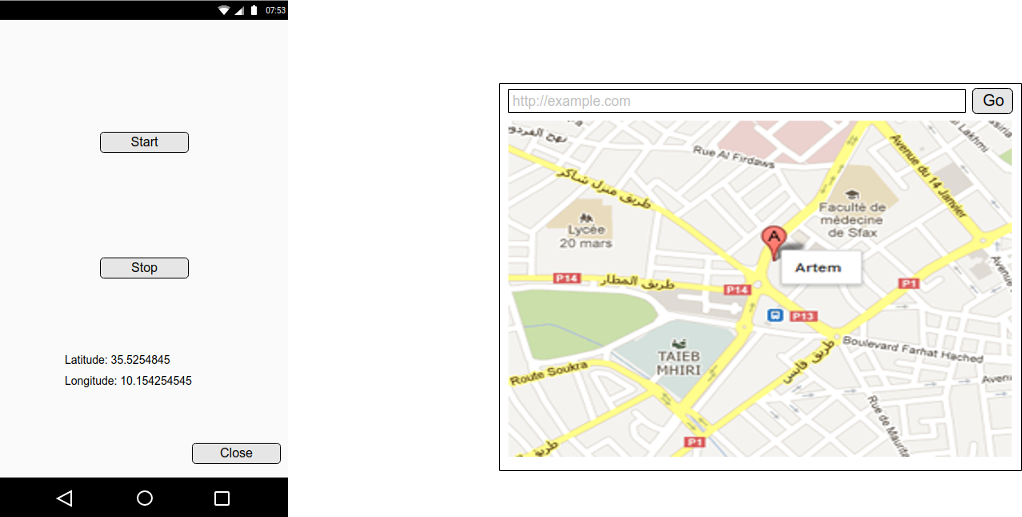
\includegraphics[width=0.7\textwidth]{sprint1-prototype}
    \caption{Prototype du produit à développer}
\label{fig:sprint1-prototype}
\end{figure}

\section{Planification de l'itération}

Pour réaliser le carnet de cette itération, nous avons décidé de diviser les
fonctionnalités en trois grandes parties:

\begin{enumerate}
    \item Une partie qui s'occupe de l'application mobile et de la détection de
        la position.
    \item Une partie  s'occupe de la partie web et l'affiche de la position
        actuelle sur une cartographie.
    \item Une partie consacrée à la réalisation de la base de données et des
        services web.
\end{enumerate}

\subsection{Backlog de l'itération}

Pour identifier la liste des tâches de cette itération, nous avons étudié un
ensemble des scénarios que nous avons les décomposés en un ensemble des cas
d'utilisations.

Concernant l'application mobile, le scénario étudié est:

\begin{enumerate}
    \item Application Android locale installée --> interface contient deux
        boutons ``Start''/``Stop''.
    \item Lancer l'application en mode en ligne (\acrshort{GPS} et internet
        activés) sinon en mode hors ligne (\acrshort{GPS} et internet
        désactivés) --> le bouton ``Start'' activé et le bouton ``Stop''
        désactivé.
    \item Appui sur le bouton ``Start'' -->  le bouton ``Start'' désactivé et
        le bouton ``Stop'' activé avec un message d'information.
    \item En cas de rupture de la connexion internet --> retourne vers le cas
        d'utilisation numéro 2.
    \item Appuis sur la bouton ``Stop'' --> le bouton ``Stop'' désactivé et le
        bouton ``Start'' activé sans messages d'information.
\end{enumerate}

Concernant la page web, le scénario étudié est:

\begin{enumerate}
    \item Lancer un navigateur (Chrome/Firefox version récente) + URL de la
        page web dans le serveur distant.
    \item Voir la carte (centrée à Sfax).
    \item Un marqueur affiché sur la carte (en position géographique de
        l'individu la plus récente).
    \item La taille de marqueur reste constante lors du zoom.
    \item L'icône du marqueur doit être personnalisée.
    \item Sans faire d'action, la position du marqueur change automatiquement
        pour montrer la dernier position de l'individu.
    \item Le curseur sur le marqueur, une fenêtre (popup) s'affiche -->
        montrant l'identifiant de la périphérique, sa longitude et sa latitude.
    \item L'icône de l'individu change sa couleur selon leur mode (en
        ligne/hors ligne).
    \item En cas de plusieurs utilisateurs --> afficher un marqueur pour
        chacun.
\end{enumerate}

On a ensuite décomposé ces cas d'utilisation en un ensemble des taches. Les
tâches à réaliser peuvent être soient des tâches de conception, de
développement, de tests, d'intégration et de documentation.

\begin{center}
    \footnotesize
    \begin{longtable}{| p{1cm} | p{5cm} | p{7cm} | p{1cm} |}
        \caption{Backlog de l'itération 1}
\label{tab:sprint1-backlog} \\

        \hline
        \textbf{Réf} & \textbf{Spécification} & \textbf{Description} & \textbf{Priorité} \\ \hline
        \endhead

        \hline \multicolumn{4}{|r|}{{Continué en page suivante$\dotsc$}} \\ \hline
        \endfoot

        \hline \hline
        \endlastfoot

        \hline
1.1 & Présentation et Configuration SVN & Présenter SVN, installer le serveur SVN et créer les répertoires & 1 \\ \hline
1.2 & Recherche sur les Services Web & Présenter les différentes Solutions des services web et choisir la meilleur solution & 1 \\ \hline
1.3 & Implémenter service Save Position & Enregistrement les coordonnées requis dans la base de données & 2 \\ \hline
1.4 & Implémenter la consommation du service Save Position & Coordonnées enregistrés instantané et continuellement dans la BD & 1 \\ \hline
1.5 & Recherche sur les spécifications de la plateforme Android & Présenter le modèle de développement Android et choisir le SDK optimale & 1 \\ \hline
1.6 & Création squelette de l'application mobile & Application fonctionnel (sans les fonctions de localisation) avec l'IHM nécessaire et l'intégration au SVN & 1 \\ \hline
1.7 & Implémenter service Get Last Position & Le serveur retourne les dernières coordonnées requis & 1 \\ \hline
1.8 & Rectification service Save Positon & Support multiple périphériques et enregistrer la date d'envoi & 2 \\ \hline
1.9 & Rectification service Get Last Position & Retourner la position du périphérique et la date de la dernière modification & 2 \\ \hline
1.10 & Affiche Multiple marqueurs & Afficher la dernière position de chaque périphérique dans la carte & 2 \\ \hline
1.11 & Affiche état du périphérique & Afficher si le périphérique est en ligne ou hors ligne & 3 \\ \hline
    \end{longtable}
\end{center}

%\begin{table}[H]
%    \centering
%    \begin{tabular}{| p{3cm} | l |}
%        \hline
%        Cas d'utilisateur & Service Save Position \\ \hline
%        Acteur & Utilisateur \\ \hline
%        Pré condition & Position non envoyée \\ \hline
%        Post condition & Position envoyée et enregistrée dans la base de données \\ \hline
%        Description du scénario &
%        \begin{minipage}{11cm}
%            \vspace*{0.2cm}
%            \begin{itemize}
%                \item L'utilisateur active le service de détection de position.
%                \item L'application détecte la position à travers le capteur \acrshort{GPS} du smartphone.
%                \item L'application envoie la position au serveur.
%                \item Le serveur vérifie et enregistre la position.
%                \item Le serveur retourne un message de confirmation d'enregistrement.
%            \end{itemize}
%        \end{minipage} \\ \hline
%        Exception & Aucune exception \\ \hline
%    \end{tabular}
%    \caption{Description du cas d'utilisation ``Service Save Position''}
%\end{table}
%
%\begin{table}[H]
%    \centering
%    \begin{tabular}{| p{3cm} | l |}
%        \hline
%        Cas d'utilisateur & Service Get Last Position \\ \hline
%        Acteur & Utilisateur \\ \hline
%        Pré condition & Position déjà enregistrée \\ \hline
%        Post condition & Position retournée \\ \hline
%        Description du scénario &
%        \begin{minipage}{11cm}
%            \vspace*{0.2cm}
%            \begin{itemize}
%                \item L'utilisateur ouvre la page du dashboard.
%                \item La page récupère la dernière position pour chaque utilisateur.
%                \item Le serveur retourne la position du chaque utilisateur.
%                \item Le page affiche un marqueur dans la position géographique de chaque utilisateur.
%                \item La page répète la récupération de la position et change la localisation du marqueur du marquer chaque 2 secondes.
%            \end{itemize}
%            \vspace{0.1cm}
%        \end{minipage} \\ \hline
%        Exception & Aucune position enregistrer pour l'utilisateur \\ \hline
%    \end{tabular}
%    \caption{Description du cas d'utilisation ``Service Get Last Position''}
%\end{table}

\subsection{Estimation de l'itération}

Avant de commencer le processus d'estimation du temps nécessaire pour la
réalisation de chaque des taches de l'itération, nous avons fixé la période
d'une itération à trois semaines. Nous avons aussi fixé le budget horaire de
chaque membre comme présenté dans le tableau~\ref{tab:sprint1-capacity}. Le
budget horaire est les heures que nous allons consacrer pour les taches de
l'implémentation du \textquote{City Watch}. Ce budget se calcule généralement
par 70\% jusqu'à 80\% de temps de disponibilité à \textquote{Djagora Academy}
vue que nous avons des autres activités et parfois des heures seront utilisées
pour assister à quelques cours.

\begin{table}[H]
    \centering
    \begin{tabular}{| c | c | c |}
        \hline
        \textbf{Membre} & \textbf{Nombre d'heures par jour} & \textbf{Budget horaire} \\ \hline
        \hline

Moez & 8 & 140\\ \hline
Rihab & 8 & 140 \\ \hline
\multicolumn{1}{c|}{} & \textbf{Total} & 280 \\ \cline{2-3}
    \end{tabular}
    \caption{Budget horaire --- Itération 1}
\label{tab:sprint1-capacity}
\end{table}

Tout les membres de l'équipe font ensuite l'estimation de temps (en point
d'histoire d'utilisateur) de chaque tâche avec le poker de planning. Les
estimations utilisées sont $\frac{1}{2}$, $1$, $2$, $3$, $5$, $8$, $13$. Les
tâches peuvent aussi être assignées aux plus qu'un seul membre.

Le tableau~\ref{tab:sprint1-estimation} représente les estimations de nos
tâches en heures ($\times2$ signifie que la tâche était assignée à deux
membres) et le membre à qui était assignée la tâche.

\begin{table}[H]
    \begin{tabular}{| l | l | l |}
        \hline
        \textbf{Spécification} & \textbf{Membre} & \textbf{Heures} \\ \hline
        \hline
Présentation et Configuration SVN & Rihab & 5 $\times$ 2 \\ \hline
Recherche sur les Services Web & Moez & 13 $\times$ 2 \\ \hline
Implémenter service Save Position & Moez & 5 \\ \hline
Implémenter la consommation du service Save Position & Rihab & 5 $\times$ 2 \\ \hline
Recherche sur les spécifications de la plateforme Android & Rihab & 13 $\times$ 2 \\ \hline
Création squelette de l'application mobile & Rihab & 13 \\ \hline
Implémenter service Get Last Position & Moez & 5 \\ \hline
Rectification service Save Positon & Moez & 5 \\ \hline
Rectification service Get Last Position & Moez & 5 \\ \hline
Affiche Multiple marqueurs & Moez & 5 \\ \hline
Affiche état du périphérique & Rihab & 5 \\ \hline
    \end{tabular}
        \caption{Nombre d'heures estimé pour la réalisation des tâches}
\label{tab:sprint1-estimation}
\end{table}

\section{Réalisation de l'application mobile}

Pour réaliser l'application mobile tracée qui contient une interface graphique
simple composée de deux boutons, nous avons choisi d'étudier la plateforme
Android et de choisir la version SDK optimale pour la réalisation de
l'application.

Android nous permet de réaliser des applications basées sur l'astuce d'activité.

\subsection{Activité}

Un utilisateur habile d'Android remarque que lors de l'exploitation d'une
application Android qu'il est en train de naviguer entre des fenêtres et
l'application n'affiche qu'une seule fenêtre à la fois. Ces fenêtres sont des
activités. On peut différencier ces activités à travers leur interface
graphique. Ceci s'applique sur la plupart des applications Android car il y a
des applications qui ne contiennent pas d'activités. Une première idée adoptée
est qu'une activité est un conteneur d'élément graphique qui constitue un
interface graphique. En effet, une activité n'est pas seulement une interface
graphique mais elle va établir les liens entre l'interface graphique et la
logique programmatique de plus l'activité contient des informations sur le
statut actuel de l'application qui s'appelle le contexte. Ce contexte permet de
faire la liaison entre le système Android et les autres activités de
l'application.

\subsubsection{États d'activités}

Le système Android met en place un système des priorités entre les
applications.  Par exemple, l'utilisateur est en train de naviguer sur internet
et d'écouter de la musique. Il reçoit un appel. Comme que l'application qui
gère les appels est une application plus prioritaire, le système pause les
autres activités pour que l'utilisateur puisse répondre à son appel. Les
activités sont gérées à partir d'un système de pile d'activités.

On peut différencier 3 états d'activité:

\begin{itemize}
    \item État Actif.
    \item État en Pause.
    \item État Arrêté.
\end{itemize}

\subsubsection{Cycle de vie d'une activité}

Une activité n'a pas de contrôle sur son état. Son état change suivant un cycle
rythmique entre le système Android et les autres applications (un système quasi
dépendant sur des priorités comme expliqué précédemment). La
figure~\ref{fig:android-activity} explique le cycle de vie d'une activité. Les
états sont représentés comme des méthodes.

% Diagram of Android activity life cycle
% Author: Pavel Seda 
% Drawing part, node distance is 1.5 cm and every node
% is prefilled with white background
\begin{figure}[H]
 \centering
 \footnotesize

\begin{tikzpicture}[node distance=1.5cm,
    every node/.style={fill=white, font=\sffamily}, align=center]
  % Specification of nodes (position, etc.)
  \node (start)             [activityStarts]              {L'activité démarre};
  \node (onCreateBlock)     [process, below of=start]          {onCreate()};
  \node (onStartBlock)      [process, below of=onCreateBlock]   {onStart()};
  \node (onResumeBlock)     [process, below of=onStartBlock]   {onResume()};
  \node (activityRuns)      [activityRuns, below of=onResumeBlock]
                                                      {Activity is running};
  \node (onPauseBlock)      [process, below of=activityRuns, yshift=-1cm]
                                                                {onPause()};
  \node (onStopBlock)       [process, below of=onPauseBlock, yshift=-1cm]
                                                                 {onStop()};
  \node (onDestroyBlock)    [process, below of=onStopBlock, yshift=-1cm] 
                                                              {onDestroy()};
  \node (onRestartBlock)    [process, right of=onStartBlock, xshift=4cm]
                                                              {onRestart()};
  \node (ActivityEnds)      [startstop, left of=activityRuns, xshift=-4cm]
                                                        {Le processus est tué};
  \node (ActivityDestroyed) [startstop, below of=onDestroyBlock]
                                                    {l'activité est arrêtée};     
  % Specification of lines between nodes specified above
  % with aditional nodes for description 
  \draw[->]             (start) -- (onCreateBlock);
  \draw[->]     (onCreateBlock) -- (onStartBlock);
  \draw[->]      (onStartBlock) -- (onResumeBlock);
  \draw[->]     (onResumeBlock) -- (activityRuns);
  \draw[->]      (activityRuns) -- node[text width=4cm]
                                   {Une autre activité s'intercole devent notre activité} (onPauseBlock);
  \draw[->]      (onPauseBlock) -- node {Notre activité n'est plus visible}
                                   (onStopBlock);
  \draw[->]       (onStopBlock) -- node {L'activité est arrêtée par le système ou l'utilisateur} (onDestroyBlock);
  \draw[->]    (onRestartBlock) -- (onStartBlock);
  \draw[->]       (onStopBlock) -| node[yshift=1.25cm, text width=3cm]
                                   {L'activité revientsur le devant de la scène}
                                   (onRestartBlock);
  \draw[->]    (onDestroyBlock) -- (ActivityDestroyed);
  \draw[->]      (onPauseBlock) -| node(priorityXMemory)
                                   {Priorité élevée $\rightarrow$ plus mémoire}
                                   (ActivityEnds);
  \draw           (onStopBlock) -| (priorityXMemory);
  \draw[->]     (ActivityEnds)  |- node [yshift=-2cm, text width=3.1cm]
                                    {L'utilisateur retourne vers l'activité}
                                    (onCreateBlock);
  \draw[->] (onPauseBlock.east) -- ++(2.6,0) -- ++(0,2) -- ++(0,2) --
     node[xshift=1.2cm,yshift=-1.5cm, text width=2.5cm]
     {L'activité revient sur le devant de la scéne}(onResumeBlock.east);

  \end{tikzpicture}
  \caption{Diagramme de cycle de vie d'activite Android}
  \captionsource{Pavel Seda, \TeX example.net [Modifié]}{http://www.texample.net/tikz/examples/android/}
  \label{fig:android-activity}
\end{figure}


%\subsubsection{Comment choisir le SDK optimale}
%
%%Une SDK permet l'application de marcher sur la version Android visé et les
%versions ultérieure il a noté de prendre en considération le taux des
%utilisateurs visé par cette application. Aussi il faut travailler avec une SDK
%digne de confidence qui n'a pas de problème ou bug qui peuvent bloquer ou
%arrêter le fonctionnement de l'application le SDK choisi doit pouvoir supporter
%les fonctionnalité offerte par l'application si on va utiliser une
%fonctionnalité qui utilise les empreinte le SDK dont on a travailler
%l'application doit supporter cette fonctionnalité lorsque le travail sur une
%application est en groupe il est mieux que tous ce groupe utilise la même SDK
%pour éviter tous problème de compatibilité et conflit entre versions de SDK
%donc il faut choisir une SDK qui est populaire en utilisation et qui est
%stable. Dans notre projet on va utiliser SDK 23 qui vise la version Android 6.0
%ayant un taux d'utilisateur qui est 4.79 \% des utilisateur d'Android notons
%que cet SDK comporte la fonctionnalité d'Android les plus récentes et qui est
%stable~\cite{android-sdk}.

La figure~\ref{fig:sprint1-android-screenshot} représente l'interface de
l'application réalisé.

Puisque la tache de l'implémentation n'était pas menée par un seul personne, on
était obligé d'introduire un système de synchronisation de notre source code.
Apache SVN était choisi pour sa simplicité, son bon support de Windows et pour
des exigences de spécification.

%\subsection{Apache Subversion}
%
%Les logiciels de gestion de versions \acrshort{VCS} nous permettent de
%conserver la chronologie des modifications du source de code, ainsi récupérer
%les version intermédiaires et les différences entre eux, et facilitent la
%collaboration au développement. Les deux logiciels de gestion de versions les
%plus répondus sont Git et Apache SVN\@.
%
%\begin{description}
%    \item [Git] Logiciel de gestion de versions distribué avec des branches
%        légères. La récupération des versions précédentes et l'enregistrement
%        des changements sont possibles sans besoin d'accès au dépôt distant car
%        chaque développeur a une copie complète du dépôt. Le modèle Fork
%        (Dupliquer), Commit (Modifier), Merge (Fusionner) a eu un grand succès
%        dans les projets libres.
%    \item [Apache SVN] Logiciel de gestion de versions centralisé. Il est connu
%        pour sa simplicité comme il n'est pas un distinct entre un dépôt local
%        vs. Dépôt distant, on faire juste une copie du dossier de travail d'une
%        version précise. Les commandes sont simples:
%        \begin{itemize}
%            \item \verb|svn checkin| \ \ vs. \ \ \verb|git commit; git push|
%            \item \verb|svn update| \ \ vs. \ \ \verb|git fetch; git rebase|
%        \end{itemize}
%        Le support du Windows est excellent surtout les outils graphiques. La
%        plus tard des fonctionnalités du SVN nécessitent l'accès au dépôt
%        (distant).
%\end{description}
%
%Apache SVN était choisi pour sa simplicité, sa bon support de Windows et pour
%des exigences de spécification.
%
%L'outil serveur choisi est VisualSVN Server pour sa simplicité d'installer et
%de configurer et pour son support du Windows.
%
%Les outils clients choisis sont:
%
%\begin{itemize}
%    \item TortoiseSVN pour l'intégration avec le système Windows.
%    \item La commande de ligne \verb|svn| est utilisée en Linux.
%    \item Le support de SVN est intégré au Android Studio et PHPStorm.
%\end{itemize}

\section{Réalisation des services web distants}

Pour réaliser les services web, nous avons étudié les différentes approches et
architectures des ces services web.

Un service web est un protocole d'interface de communication et l'échange de
données entre applications et systèmes hétérogènes à distance en utilisant les
technologies Web (HTTP dans notre cas). Les différentes variantes des
architectures des services web sont:

\begin{itemize}
    \item Architecture orientée RPC (ex: XML-RPC, SOAP, JSON-RPC):
        \begin{itemize}
            \item Meilleur pour présenter des actions et commandes.
        \end{itemize}
    \item Architecture orientée Ressources (ex: RESTful):
        \begin{itemize}
            \item Représenter les données sous formes des ressources.
            \item Utiliser les méthodes HTTP pour modifier/créer/lire/supprimer
                les données.
            \item Utiliser les paramètres d'URL pour passer des paramètres.
            \item Sans état.
            \item Meilleur pour modéliser un domaine et entités.
        \end{itemize}
\end{itemize}

Le choix final de l'architecture du service web à suivre était l'architecture
RESTful.

Avant de commencer la conception et l'implémentation des services web, un
ensemble des exigences ont été définies:

\begin{description}
    \item [Portabilité] Le système doit support la différence en zone du temps
        et en internalisation, la format de présentation des données
        géographiques et sa précision.
    \item [Stabilité] L'implémentation doit vérifier la structure des données
        reçues, la disponibilité des champs obligatoires et leurs formats.
\end{description}


\subsection{Conception}

La figure~\ref{fig:sprint1-webservices-usecase} décrit le diagramme
de cas d'utilisation qui regroupe les scénarios de localisation d'individu.

\begin{figure}[H]
    \centering
    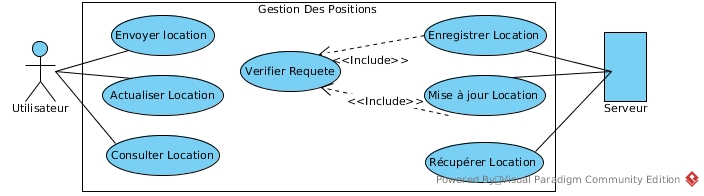
\includegraphics[width=1\textwidth]{sprint1-webservices-usecase}
    \caption{Diagramme de cas d'utilisation du services web --- Itération 1}
\label{fig:sprint1-webservices-usecase}
\end{figure}

La figure~\ref{fig:sprint1-webservices-post-sequence} décrit le diagramme de
séquence du service \textquote{Post Position} qui représente les scénarios de
l'envoi de la position. L'utilisateur ouvre l'application mobile et active la
localisation. L'application capture la position à travers le GPS et l'envoie au
serveur. Le serveur vérifie le chemin de la requête, sa format et son contenu
puis enregistre la position de l'individu. L'application renvoie la position en
changement de la localisation pour que le serveur la met à jour.

\begin{figure}[H]
    \centering
    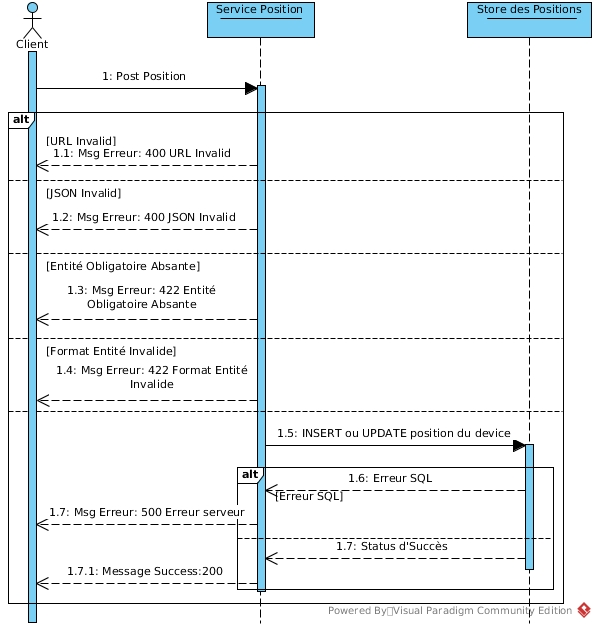
\includegraphics[width=1\textwidth]{sprint1-webservices-post-sequence}
    \caption{Diagramme de séquence du service Post Position --- Itération 1}
\label{fig:sprint1-webservices-post-sequence}
\end{figure}

La figure~\ref{fig:sprint1-webservices-get-sequence} décrit le diagramme de
séquence du service \textquote{Get Position} qui représente les scénarios du
récupération de la position. L'utilisateur visite la page web du Dashboard pour
consulter sa dernière position.  Le système récupère la dernière position des
périphériques chaque 2 secondes et met à jour la position géographique des
marqueurs dans la cartographie et leurs états à hors ligne s'ils n'ont aucun
mise à jour du position depuis 60 secondes. Pour chaque requête de
récupération, le serveur vérifie la présence de la position du périphérique et
retourne sa dernière position enregistrée.

\begin{figure}[H]
    \centering
    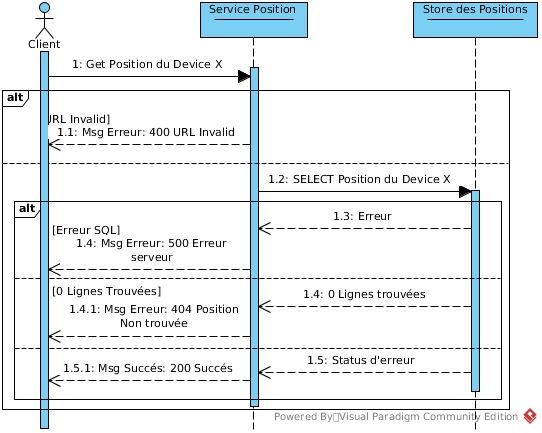
\includegraphics[width=1\textwidth]{sprint1-webservices-get-sequence}
    \caption{Diagramme de séquence du service Get Position --- Itération 1}
\label{fig:sprint1-webservices-get-sequence}
\end{figure}

Le schéma~\ref{fig:sprint1-webservices-class} présente le diagramme des classes
du service web dans cette itération.

\begin{figure}[H]
    \centering
    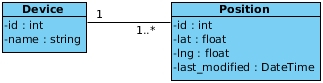
\includegraphics[width=0.6\textwidth]{sprint1-webservices-class}
    \caption{Diagramme de classe du service web --- Itération 1}
\label{fig:sprint1-webservices-class}
\end{figure}

Le schéma de la base de données de cette itération est dans
l'annexe~\ref{sec:sprint1-database}.

\subsection{Services web}

Dans première phase, nous avons implémenté les méthodes POST et GET du
ressource Position. L'architecture résultante est documentée dans
l'annexe~\ref{appendix:sprint1-position-post-doc}
et~\ref{appendix:sprint1-position-get-doc}.

Nous avons essayé d'adresser les différentes mises en normes:

\subsubsection{Probabilité}

Nous avons utilisé la format standardisée JSON~\cite{ECMA-404} pour le
transfert de données ce qui assure la portabilité des représentations des
différents types des données (nombres, booléens, strings, \ldots) indépendant
du l'internationalisation (séparateur décimal, \verb|true| vs. \verb|True| vs.
\verb|vrai| vs. \verb|yes| vs. \verb|y|, \ldots).

Pour la représentation des dates dans le content du requêtes HTTP, nous avons
utilisé le format RFC3339~\cite{RFC3339} (basé sur ISO8601~\cite{ISO8601} pour
l'utilisation dans les protocoles du Web) avec UTC comme la zone du temps par
défaut, ex: \verb|2005-08-15T15:52:01Z|.

Pour les en-têtes du requêtes HTTP, le format de représentation des dates est
RFC1123~\cite{RFC1123}, ex: \verb|Mon, 15 Aug 2005 15:52:01 +0000|.

Le format de la présentation des positions géologique (latitude et longitude)
choisie est la même représentation des nombres en JSON avec une précision
jusqu'à 14 chiffres après le séparateur décimal. Les valeurs envoyées doivent
respecter l'intervalle des diffèrent entités géologiques ($latitude \in [-90,
90]$, $longitude \in [-180, 180]$)

\subsubsection{Stabilité}

Pour assurer la stabilité d'un service web, nous avons vérifié la validité de
contenu reçu même si envoyé depuis un source de confiance avant de les
utiliser. La vérification inclut le test de disponibilité des entités
obligatoires et le test de leurs formats.

\section{Revue de cette itération}

À la fin de l'itération, notre équipe et le \textquote{Product Owner} invitées
se réunissent pour effectuer la revue de sprint, qui dure au maximum deux
heures.

L'objectif de la revue de l'itération est de valider l'incrément de produit qui
a été réalisé pendant cette itération. L'équipe énonce les éléments du backlog
en début de sprint, et présente les tâches finies (complètement réalisées).

\subsection{Produit de l'itération}

A la fin de l'itération 1, nous avons un premier produit partiel permettant de
suivre la position des multiples smartphones et les afficher dans la carte de
notre site web.

\subsubsection{Page Web \textquote{Dashboard}}

La figure~\ref{fig:sprint1-dashboard-screenshot} affiche la position des
individus et son état.

\begin{itemize}
    \item \textit{Marqueur en Vert}: Périphérique en ligne.
    \item \textit{Marqueur en Rouge}:Périphérique en hors ligne.
\end{itemize}

\begin{figure}[H]
    \centering
    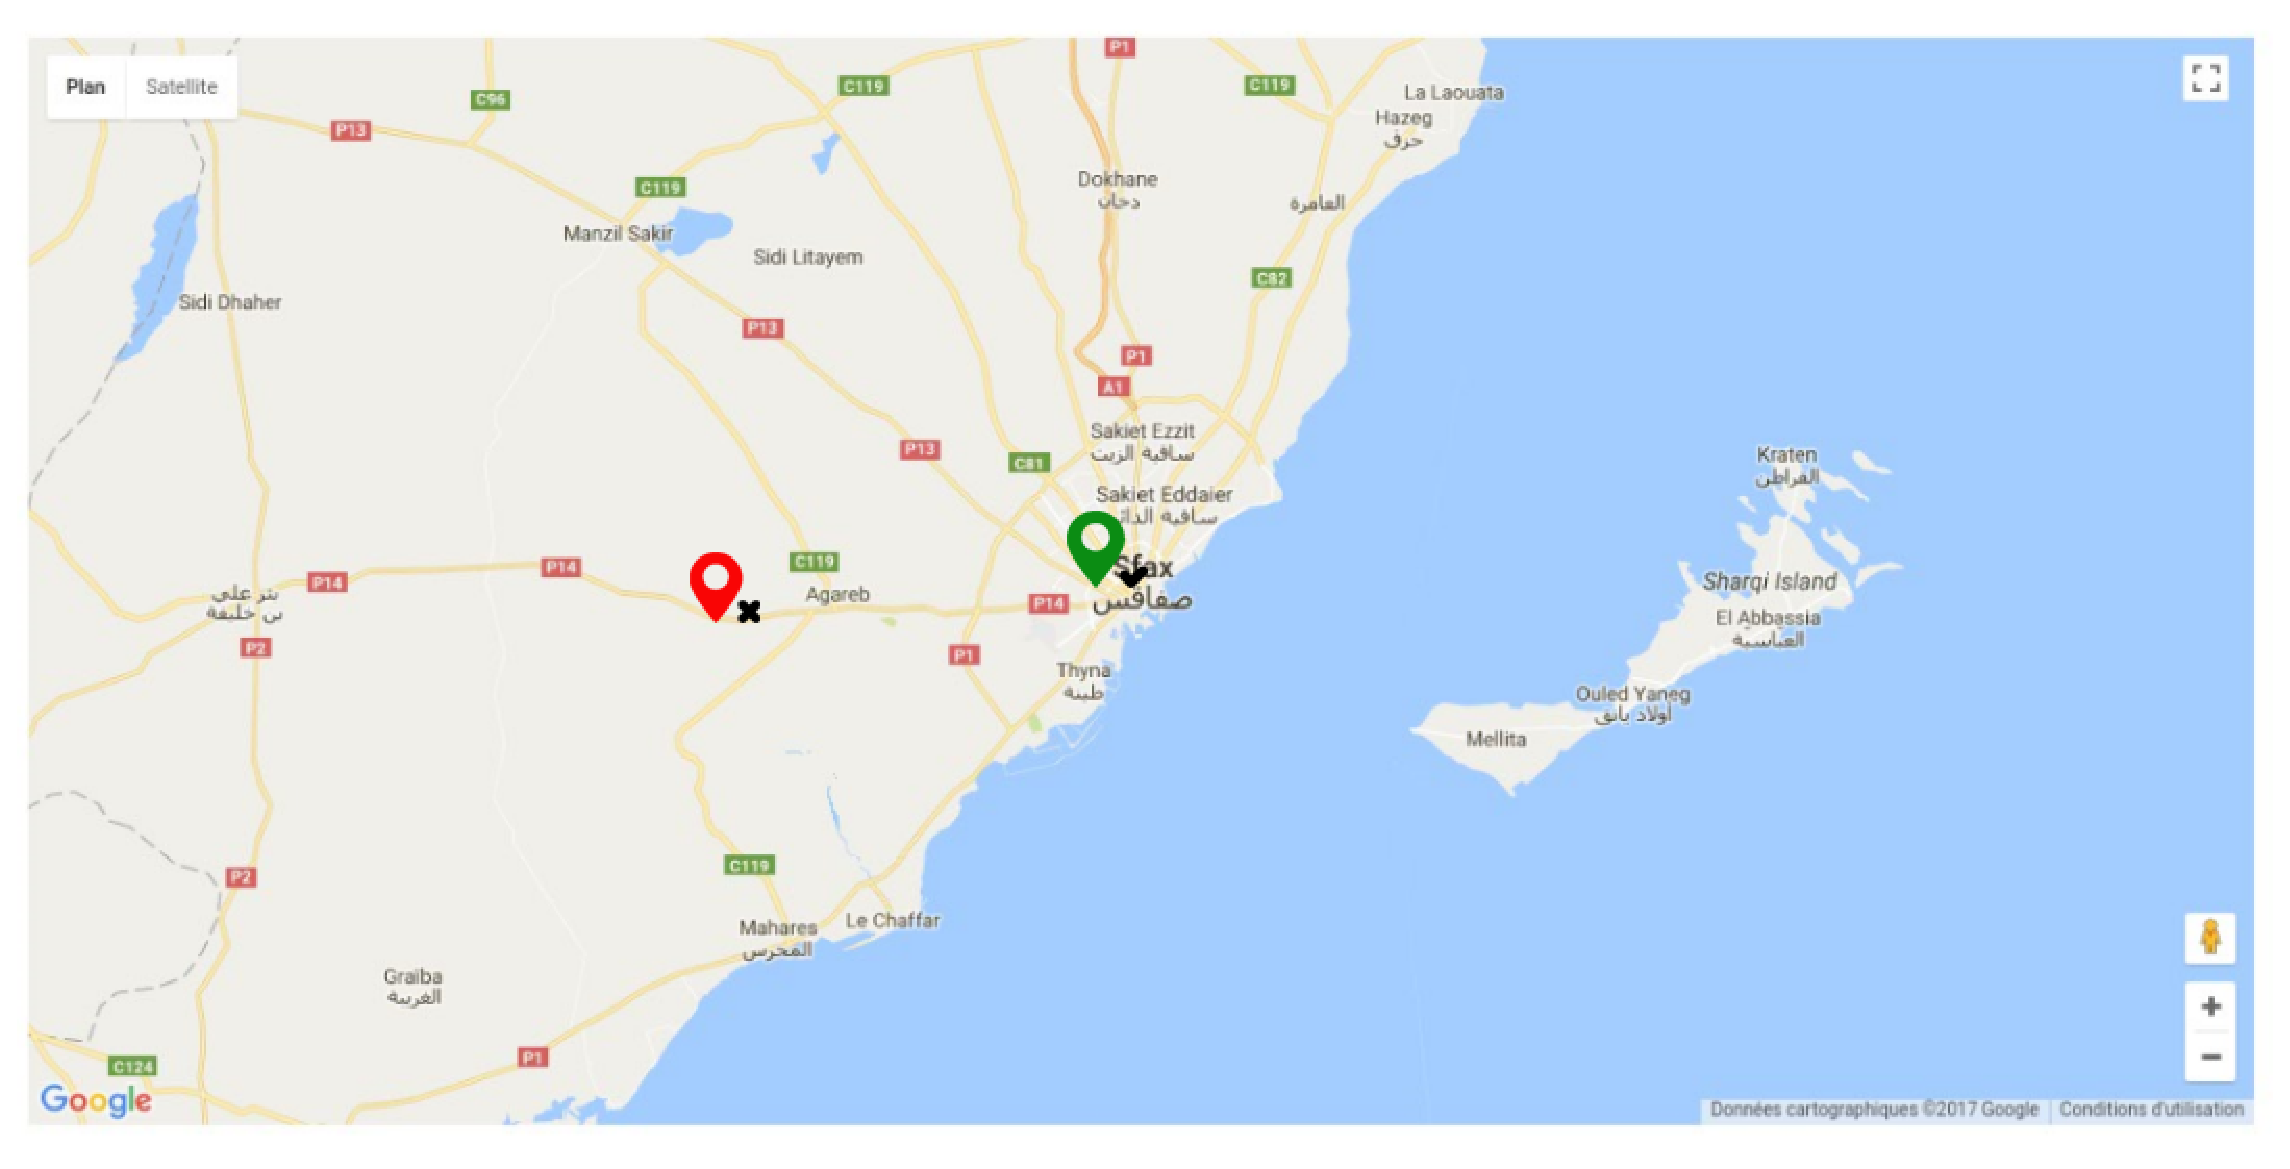
\includegraphics[width=0.8\textwidth]{sprint1-dashboard-screenshot}
    \caption{Capture écran de la page web de l'itération 1}
\label{fig:sprint1-dashboard-screenshot}
\end{figure}

\subsubsection{Application Android}

\begin{figure}[H]
    \centering
    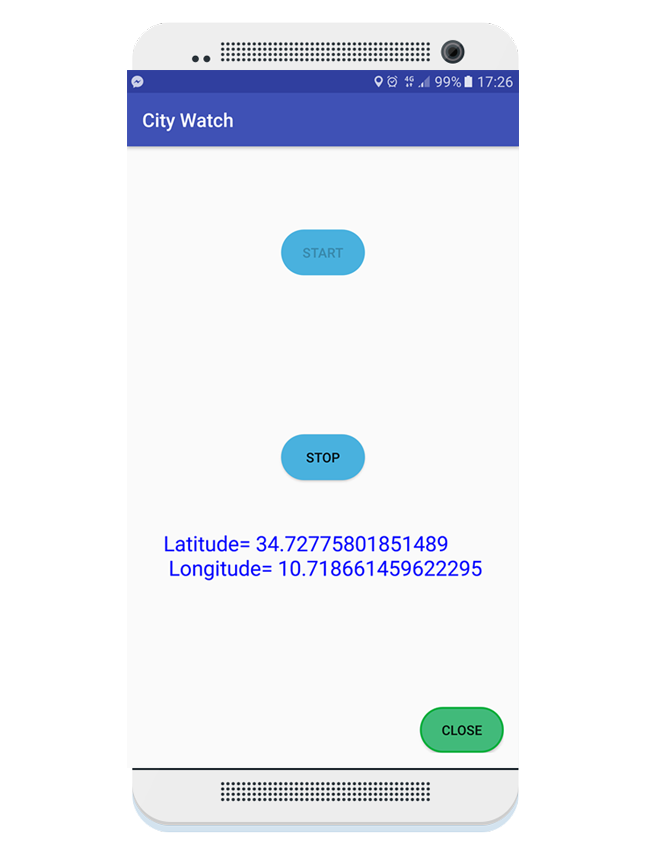
\includegraphics[width=0.35\textwidth]{sprint1-android-screenshot}
    \caption{Capture écran de l'application dans l'itération 1}
\label{fig:sprint1-android-screenshot}
\end{figure}

L'application Android de cette itération est composée de trois boutons
``Start'', ``Stop'' et ``Close''.  Le clique sur le bouton ``Start'' active la
détection continuelle de la position qui nécessite la disponibilité de
l'Internet et du \acrshort{GPS}.  Le clique sur le bouton ``Stop'' désactive la
détection de la position.

\subsection{Avis du Product Owner}

Le Product Owner était ravi des résultats de cette première itération. Il a
validé donc notre travail et nous a encouragé pour l'élaboration des suivantes
itérations.

\subsection{Burndown chart}

La figure~\ref{fig:sprint1-burndown} présente une vue d'ensemble sur le progrès
de notre travail au cours de l'itération par rapport au progrès idéal.

\usetikzlibrary{plotmarks}

\begin{figure}
\centering
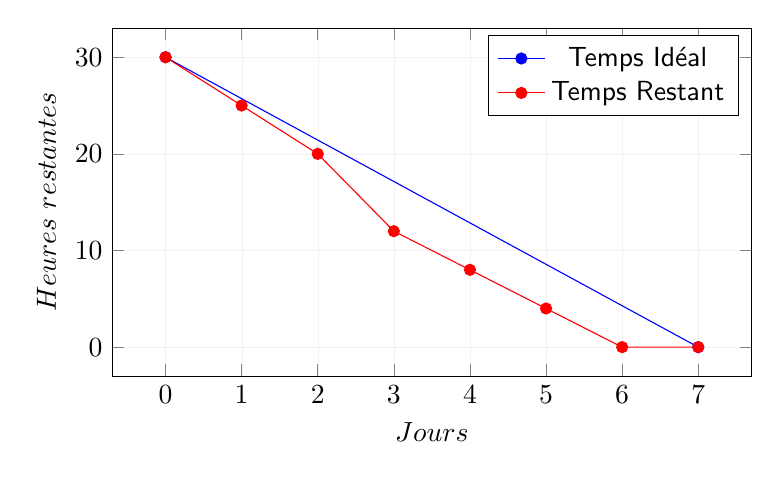
\begin{tikzpicture}[y=.2cm, x=.7cm,font=\sffamily]
\begin{axis}[
xlabel=$Jours$,
ylabel=$Heures\ restantes$,
grid=both,
grid style={line width=.1pt, draw=gray!10},
width=0.8\textwidth,
height=6cm,
%major grid style={line width=.2pt,draw=gray!50},
]
\addplot[color=blue,mark=*] coordinates {
        (0,30)
        (7, 0)
    };
    \addlegendentry{Temps Idéal}

    \addplot[mark=*,red] plot coordinates {
        (0, 30)
        (1, 25)
        (2, 20)
        (3, 12)
        (4, 8)
        (5, 4)
        (6, 0)
        (7, 0)
    };
    \addlegendentry{Temps Restant}
\end{axis}
\end{tikzpicture}
\caption{Graphique d'avancement - Itération 1}
\end{figure}


\subsection{Rétrospectif de l'itération}

À la fin de la réunion, les membres de l'équipe ont fait un rétrospectif
interne pour créer un plan d'amélioration qui sera mis en place au cours de
l'itération suivante.  Nous avons décidé de suivre quelques règles pour assurer
la qualité du code.

\begin{itemize}
    \item Activer le mode strict du PHP et changer le mode de traitement des
        erreurs au déclenchement des exceptions si possible (PDO, \ldots).
        Activer le mode strict du JavaScript aussi.
    \item Utiliser des analyseurs statiques du code: PHP\_CodeSniffer, PHPLint
        et ESLint pour détecter les erreurs formelles de programmation ou de
        conception.
    \item Documenter chaque fonction, classe, constante et variable global. On
        a utilisé PHPDoc, apiDoc et JSDoc pour documenter le code PHP, l'api
        RESTful et le code JavaScript respectivement. Pour rédiger les
        recherches, les présentations et les autres documentations, \LaTeX{}
        était préféré avec la possibilité d'utiliser Markdown pour la
        simplicité de sa syntaxe.
    \item Écrire les tests unitaires pour les fonctions et les classes selon la
        technique \acrshort{TDD}. On a autorisé l'écrire des tests unitaires
        après le développement du code. Les outils utilisés sont PHPUnit pour
        PHP et Mocha/Chai pour JavaScript.
\end{itemize}

Le tableau~\ref{tab:sprint1-evaluation} présente le pourcentage de réalisation
de nos tâches de cette itération.

\begin{center}
    \begin{longtable}{| l | l |}
        \caption{Liste des tâches réalisées de la première itération}
\label{tab:sprint1-evaluation} \\

        \hline
        \textbf{Les tâches} & \textbf{Taux de réalisation} \\ \hline
        \endhead

        \hline \multicolumn{2}{|r|}{{Continué en page suivante$\dotsc$}} \\ \hline
        \endfoot

        \hline \hline
        \endlastfoot

        \hline
Présentation et Configuration SVN & Effectué 100\% \\ \hline
Recherche sur les Services Web & Effectué 100\% \\ \hline
Implémenter service Save Position & Effectué 100\% \\ \hline
Implémenter la consommation du service Save Position & Effectué 100\% \\ \hline
Recherche sur les spécifications de la plateforme Android & Effectué 100\% \\ \hline
Création squelette de l'application mobile & Effectué 100\% \\ \hline
Implémenter service Get Last Position & Effectué 100\% \\ \hline
Rectification service Save Positon & Effectué 100\% \\ \hline
Rectification service Get Last Position & Effectué 100\% \\ \hline
Affiche Multiple marqueurs & Effectué 100\% \\ \hline
Affiche état du périphérique & Effectué 100\% \\ \hline
    \end{longtable}
\end{center}

\section*{Conclusion}
\addcontentsline{toc}{section}{Conclusion}

À la fin de cette itération, nous avons un prototype fonctionnel dont on peut
baser notre future travail.
